\documentclass{article}

\usepackage{fancyhdr}
\usepackage[letterpaper,margin=0.45in,includehead,includefoot,headheight=14pt,headsep=6pt]{geometry}
\usepackage{microtype}
\usepackage{multicol}
\usepackage{enumitem}
\usepackage{amsmath,amssymb}
\usepackage[hidelinks]{hyperref}
\usepackage{graphicx}
\usepackage[export]{adjustbox}
\usepackage{tikz}
\usepackage{titlesec}
\usetikzlibrary{calc}

\setlength{\columnsep}{0.2in}
\setlength{\parindent}{0pt}
\setlength{\parskip}{2pt}
\setlist{nosep,leftmargin=*}
\setlength{\abovedisplayskip}{3pt}
\setlength{\belowdisplayskip}{3pt}
\setlength{\emergencystretch}{1em}
\titlespacing*{\section}{0pt}{5pt}{2pt}
\titlespacing*{\subsection}{0pt}{2pt}{0pt}

\pagestyle{fancy}
\fancyhf{}
\fancyhead[L]{\textbf{Sets Core}}
\fancyhead[R]{Name: \rule{2.2in}{0.4pt}}
\fancyfoot[C]{\thepage}
\renewcommand{\headrulewidth}{0.4pt}

\newcommand{\vennworkspace}{%
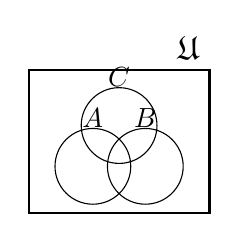
\begin{tikzpicture}[scale=0.37]
    \draw[thick] (-2.2,-1.6) rectangle (4.0,3.3) node[above left]{\large $\mathfrak U$};
    \def\rad{1.3}
    \coordinate (A) at (0,0);
    \coordinate (B) at (1.8,0);
    \coordinate (C) at (0.9,1.4);
    \draw (A) circle (\rad);
    \draw (B) circle (\rad);
    \draw (C) circle (\rad);
    \node at ($(A)+(0,\rad+0.35)$) {$A$};
    \node at ($(B)+(0,\rad+0.35)$) {$B$};
    \node at ($(C)+(0,\rad+0.35)$) {$C$};
\end{tikzpicture}%
}

\begin{document}
\small
\raggedcolumns

\textbf{Practice source.} A supervised attempt lasts 20 minutes and contains
five problems: one from each section A--E. Each labeled problem is one scoring
unit, including all of its required parts. Four fully correct problems earn
\textbf{Meets}; five earn \textbf{Exceeds}. Every retake uses a complete new
five-problem form, including a retake after Meets to earn Exceeds.

\textbf{Directions.} Show enough work to make your reasoning clear. A bare
answer earns credit only when the prompt asks for a list or classification.
Complements are taken relative to the stated universal set.

\section*{A. Set Language and Finite Constructions (Rosen 2.1)}

For each problem, complete every part.

\begin{multicols}{2}
\subsection*{A.1}
Let $S=\{x\in\mathbb Z:-2\le x<3\}$ and $T=\{-2,2\}$.
\begin{enumerate}[label=(\alph*)]
  \item Write $S$ in roster notation.
  \item Decide whether $T\subseteq S$ and whether $T\in S$.
  \item List every element of $\mathcal P(T)$.
\end{enumerate}

\subsection*{A.2}
Let $S=\{x\in\mathbb Z:-4\le x\le4\text{ and }x\text{ is even}\}$ and
$T=\{-2,4\}$.
\begin{enumerate}[label=(\alph*)]
  \item Write $S$ in roster notation.
  \item Decide whether $T\subseteq S$ and whether $-2\in T$.
  \item List $T\times\{0,1\}$.
\end{enumerate}

\subsection*{A.3}
Let $S=\{x\in\mathbb Z^+:x\mid12\}$ and $T=\{2,3\}$.
\begin{enumerate}[label=(\alph*)]
  \item Write $S$ in roster notation.
  \item Decide whether $T\subseteq S$ and whether $T\in\mathcal P(S)$.
  \item List every element of $\mathcal P(T)$.
\end{enumerate}

\subsection*{A.4}
Let $S=\{n^2:n\in\mathbb Z,-2\le n\le2\}$ and $T=\{0,1\}$.
\begin{enumerate}[label=(\alph*)]
  \item Write $S$ in roster notation, without repetitions.
  \item Decide whether $T\subset S$ and whether $2\in S$.
  \item List $T\times S$.
\end{enumerate}

\subsection*{A.5}
Let $S=\{x\in\mathbb Z:|x|\le2\}$ and $T=\{-1,1\}$.
\begin{enumerate}[label=(\alph*)]
  \item Write $S$ in roster notation.
  \item Decide whether $T\subseteq S$ and whether $\{0\}\in S$.
  \item List every element of $\mathcal P(T)$.
\end{enumerate}
\end{multicols}

\section*{B. Set Operations and Venn Regions (Rosen 2.2)}

For each formula, shade exactly the set of points $x\in\mathfrak U$ for which
the formula is true. Then write the shaded region using only union,
intersection, complement, and set difference.

\begin{multicols}{2}
\subsection*{B.1}
$(x\in A\setminus B)\lor(x\in C)$
\begin{center}\vennworkspace\end{center}

\subsection*{B.2}
$(x\in \overline A)\lor(x\in B\cup C)$
\begin{center}\vennworkspace\end{center}

\subsection*{B.3}
$(x\in A\cup B)\to(x\in C)$
\begin{center}\vennworkspace\end{center}

\subsection*{B.4}
$((x\in A)\to(x\in B))\land(x\in C)$
\begin{center}\vennworkspace\end{center}

\subsection*{B.5}
$(x\in A)\leftrightarrow(x\in B\setminus C)$
\begin{center}\vennworkspace\end{center}
\end{multicols}

\clearpage
\section*{C. Relations as Subsets of Cartesian Products (Rosen 2.1, 2.3)}

For each plotted relation $R\subseteq X\times Y$, where
$X=Y=\{1,2,3\}$:
\begin{enumerate}[label=(\alph*)]
  \item list $R$ as a set of ordered pairs;
  \item decide whether each stated quantified proposition is true or false; and
  \item decide whether $R$ is a function from $X$ to $Y$. If it is, classify it
  as injective, surjective, both, or neither. If it is not, identify an input
  with either no output or more than one output.
\end{enumerate}

\begin{multicols}{2}
\subsection*{C.1}
Evaluate $\forall x\,\exists!y\,((x,y)\in R)$ and
$\forall y\,\exists!x\,((x,y)\in R)$.
\begin{center}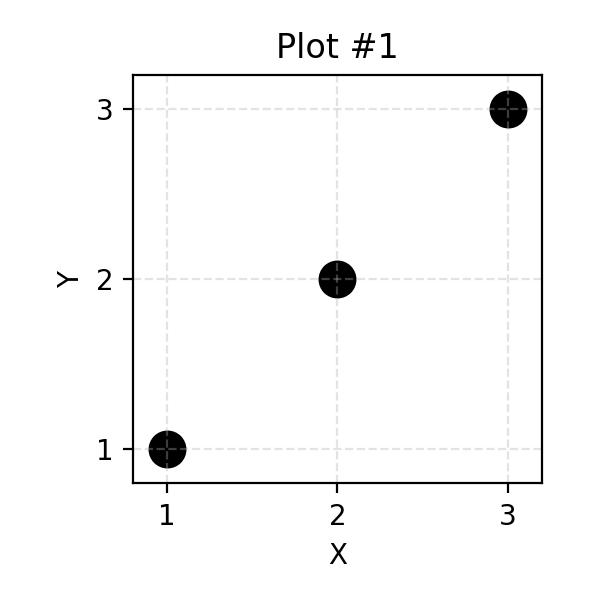
\includegraphics[width=0.52\linewidth]{../../images/set_plot1.jpg}\end{center}

\subsection*{C.2}
Evaluate $\forall x\,\exists y\,((x,y)\in R)$ and
$\exists x\,\forall y\,((x,y)\in R)$.
\begin{center}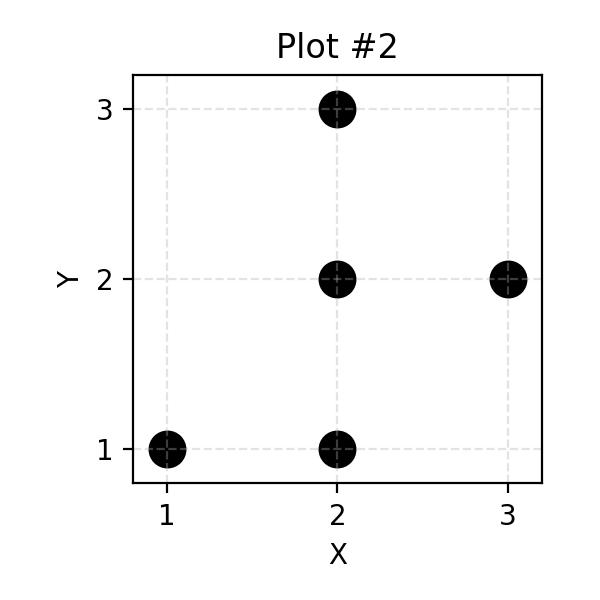
\includegraphics[width=0.52\linewidth]{../../images/set_plot2.jpg}\end{center}

\subsection*{C.3}
Evaluate $\forall y\,\exists x\,((x,y)\in R)$ and
$\exists y\,\forall x\,((x,y)\in R)$.
\begin{center}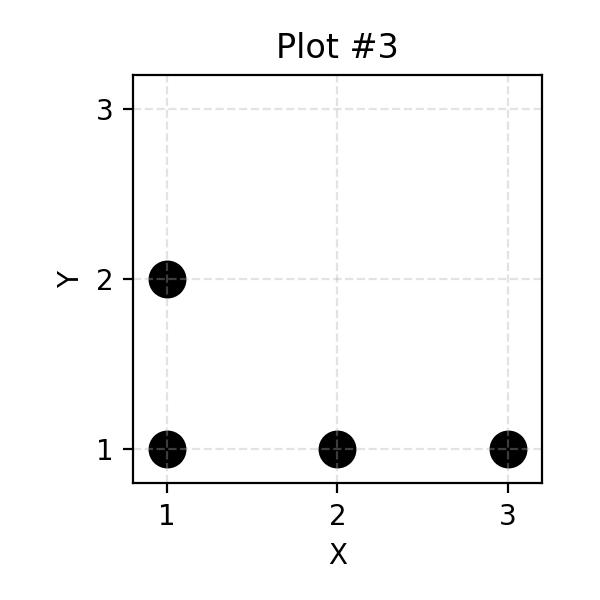
\includegraphics[width=0.52\linewidth]{../../images/set_plot3.jpg}\end{center}

\subsection*{C.4}
Evaluate $\forall x\,\exists!y\,((x,y)\in R)$ and
$\exists x\,\forall y\,((x,y)\in R)$.
\begin{center}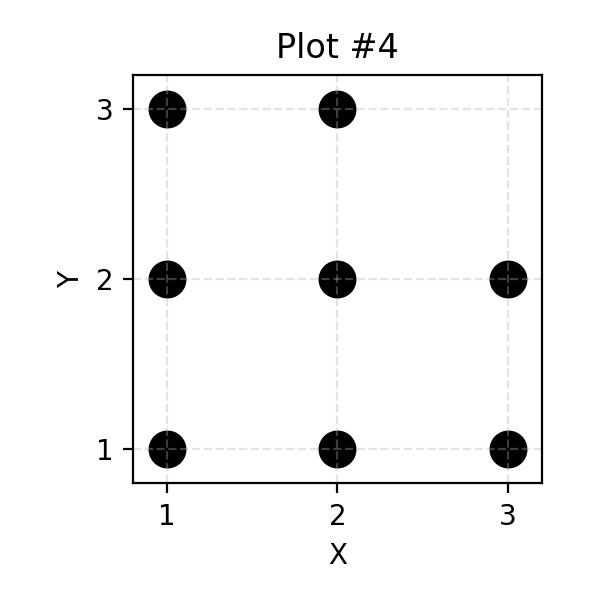
\includegraphics[width=0.52\linewidth]{../../images/set_plot4.jpg}\end{center}

\subsection*{C.5}
Evaluate $\forall y\,\exists!x\,((x,y)\in R)$ and
$\exists y\,\forall x\,((x,y)\in R)$.
\begin{center}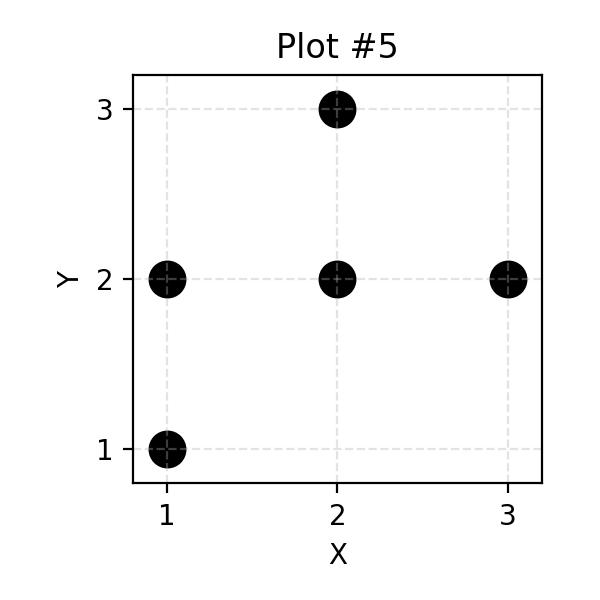
\includegraphics[width=0.52\linewidth]{../../images/set_plot5.jpg}\end{center}
\end{multicols}

\clearpage
\section*{D. Functions, Images, and Preimages (Rosen 2.3)}

\begin{multicols}{2}
\subsection*{D.1}
Let $A=\{1,2,3,4\}$ and $B=\{a,b,c\}$. Define $f:A\to B$ by
$f(1)=a$, $f(2)=b$, $f(3)=b$, and $f(4)=c$.
\begin{enumerate}[label=(\alph*)]
  \item Find $f(\{1,3,4\})$ and $f^{-1}(\{a,b\})$.
  \item Classify $f$ as injective, surjective, both, or neither. Justify your
  answer.
\end{enumerate}
\vspace{0.35in}

\subsection*{D.2}
Let $g:\mathbb Z\to\mathbb Z$ be $g(n)=n+5$.
\begin{enumerate}[label=(\alph*)]
  \item Find $g(\{-1,0,2\})$ and $g^{-1}(\{4,7\})$.
  \item Classify $g$ as injective, surjective, both, or neither. Justify both
  properties.
\end{enumerate}
\vspace{0.35in}

\subsection*{D.3}
Let $h:\mathbb Z\to\mathbb Z$ be $h(n)=n^2$.
\begin{enumerate}[label=(\alph*)]
  \item Find $h(\{-2,-1,0,2\})$ and $h^{-1}(\{0,1,4\})$.
  \item Classify $h$ as injective, surjective, both, or neither. Give concrete
  witnesses for any failed property.
\end{enumerate}
\vspace{0.35in}

\subsection*{D.4}
Let $k:\mathbb Z\to\mathbb Z$ be $k(n)=2n$.
\begin{enumerate}[label=(\alph*)]
  \item Find $k(\{-1,0,1\})$ and $k^{-1}(\{-2,0,4\})$.
  \item Classify $k$ as injective, surjective, both, or neither. Justify your
  answer.
\end{enumerate}
\vspace{0.35in}

\subsection*{D.5}
Let $q:\mathbb N_0\to\{m^2:m\in\mathbb N_0\}$ be $q(n)=n^2$, where
$\mathbb N_0=\{0,1,2,\ldots\}$.
\begin{enumerate}[label=(\alph*)]
  \item Find $q(\{0,2,3\})$ and $q^{-1}(\{1,16\})$.
  \item Classify $q$ as injective, surjective, both, or neither. Explain how
  the declared domain and codomain affect the answer.
\end{enumerate}
\vspace{0.35in}
\end{multicols}

\clearpage
\section*{E. Prove or Refute a Set/Function Claim (Rosen 2.1--2.3)}

For each problem, decide whether the claim is true for all sets and functions
of the stated types. If it is true, prove it by following an arbitrary element.
If it is false, give a specific finite counterexample and compute both sides.

\begin{multicols}{2}
\subsection*{E.1}
If $f:X\to Y$ and $U,V\subseteq X$, then
\[
f(U\cup V)=f(U)\cup f(V).
\]
\vspace{0.9in}

\subsection*{E.2}
If $f:X\to Y$ and $U,V\subseteq X$, then
\[
f(U\cap V)=f(U)\cap f(V).
\]
\vspace{0.9in}

\subsection*{E.3}
If $f:X\to Y$ and $P,Q\subseteq Y$, then
\[
f^{-1}(P\cap Q)=f^{-1}(P)\cap f^{-1}(Q).
\]
\vspace{0.9in}

\subsection*{E.4}
For all sets $A,B,C$,
\[
(A\cup B)\times C=(A\times C)\cup(B\times C).
\]
\vspace{0.9in}

\subsection*{E.5}
For all sets $A,B,C$, if $A\cup B=A\cup C$, then $B=C$.
\vspace{0.9in}
\end{multicols}

\end{document}
